% https://tex.stackexchange.com/a/55242/173708
% arr: reindent; change page size
\documentclass[border=10]{standalone}
\usepackage{tikz}
\usetikzlibrary{positioning}


\newcommand{\symbolA}{
	\tikz \draw[red] (0,0)--(0,0.2)--(0.2,0.2)--(0.2,0.4)--(0.4,0.4);
}

\newcommand{\symbolB}{
	\tikz[y={(0,-1)}] \draw[blue] (0,0)--(0,0.2)--(0.2,0.2)--(0.2,0.4)--(0.4,0.4);
}

\newcommand{\symbolC}{
	
\begin{tikzpicture}
		\draw[fill=green] (0,0) circle (0.2cm);
	\end{tikzpicture}
}


\begin{document}

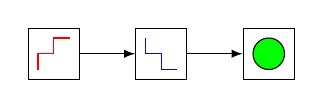
\begin{tikzpicture}
	\node[draw](A) at (0,0){\symbolA};
	\node[draw, right=2em of A] (B) {\symbolB};
	\node[draw, right=2em of B] (C) {\symbolC};
	\draw[-latex] (A) -- (B);
	\draw[-latex](B) -- (C);
\end{tikzpicture}

\end{document}